\documentclass[10pt,conference,compsocconf]{IEEEtran}

\usepackage{hyperref}
\usepackage{graphicx}	% For figure environment
\usepackage{array}
\usepackage{diagbox}
\usepackage{amssymb}
\usepackage{amsmath}
\usepackage[right=1cm,left=1cm,top=2cm,bottom=2cm]{geometry}
\begin{document}
\title{Machine learning - Project 1 report}
\author{Group 21 -- \textit{Volodymyr Loyko, Shiyue Nie, Thomas Sanchez}}

\maketitle

\section{Introduction}
This report overviews the way we approached the problem of the classification of the Higgs Boson. We first cover the transformation that we applied to the data, then present the different methods we applied to try to solve the problem and finally discuss in greater detail our best submission.

\section{Formatting the Data}
The data we were given about the Higgs Boson contains 30 columns of measurements, some of which are NaNs. In order to avoid biased results, it is necessary to clean those NaNs(either $-999$ or $0$) before utilizing the data. We will briefly discuss the techniques we used to achieve this.

\subsubsection{Counting the NaNs}
An NaN in a given column could be correlated to the measurement of a Higgs Boson.  Adding a column which keeps track of the number of NaNs found in each row to the data allows us to safely remove NaNs without losing the information that they represent. 

\subsubsection{Removing the NaNs}
For each column that contains an NaN we first retrieved all the non-NaN points in the column and find their median. We then simply replaced the NaNs with this value. We use the median and not the mean because the it is robust to outliers. Imagine having all the “valid” points in the region −1 to 1, the NaNs as −999 and an outlier at a very large value. This outlier would have a large effect on the mean of this example data, while having no effect on the median.

\subsubsection{Standardization of the Data}
The third step in the formatting sequence of the data is to standardize it. Having the gradient with the same magnitude in every direction yields a faster convergence for the methods that make use of gradient descent, like logistic regression. It is also useful for when we wish to construct a polynomial basis, as it keeps the large values of our data set bounded. It is important to note that in the case where a column has standard deviation of 0, i.e. all of its values are the same, we remove it from the data, as it contains no useful information. 

\subsubsection{Polynomial basis} 
Finally we take a polynomial basis of degree D for the data. We did not add the cross terms of the form $x_1x_2x_3$ for polynomials of degree three as this would have given far too many features for our model to fit. For a basis of degree $D$ and an input with $M$ features, our polynomial basis was of the form 
\begin{equation}
\left[1 ~ \mathbf{x}_1 \cdots \mathbf{x}_N ~\mathbf{x}_1^2 \cdots \mathbf{x}_N^2 ~ \mathbf{x}_1^D \cdots \mathbf{x}_N^D \right] \mbox{ where } \mathbf{x}_i \in \mathbb{R}^M
\end{equation}
\subsubsection{Additional note}
We apply the same transformation to our testing set, yet we do not recompute the median, mean and standard deviation. Instead we apply the values that we had found for the training set, otherwise we will end up with a biased result. 
\section{Results}
\subsection{Methodology}
The methodology we followed to obtain our results was an extensive use of the cross validation while varying all the other parameters ($\lambda$ in the ridge regression as well as the polynomial degree) we had in a grid-search fashion. We would then choose the combination that yielded the minimal error, i.e. the smallest percentage of classification error. We did not iterate on $\gamma$ for the iterative methods, as the $\gamma$ will only change the speed of convergence of the method. Instead we tried to pick a $\gamma$ that seemed to work well and extended the number of maximal iterations until convergence.

\subsection{General results and comments}
Let us now present quickly some results that we obtained with each method. Note that, as the Ridge Regression stood quickly out as the best for our purpose, we did not extensively try to use the other methods, hence the results shown here for all other methods could easily be improved, and they are just present here for comparison's sake.
\begin{table}[!h]
	\centering
	\begin{tabular}{c||c|c|c|c|c|c}
		\textbf{Method used} & GD & SGD & LS & RR & LR & RLR  \\
		\hline
		\textbf{Accuracy ($\%$)} & $70.0$&$70.1$&$71.9$&$81.8$&$77.4$&$69.0$\\
		\hline
		\textbf{Degree} & $1$ &$1$&$1$&$12$&$2$&$3$\\
		\hline
		$\mathbf{\gamma}$ & $2^{-6}$&$2^{-12}$&\diagbox{}&\diagbox{}&$10^{-8}$&$10^{-6}$\\
		\hline
		\textbf{max\_iters} & $2000$&$2000$&\diagbox{}&\diagbox{}&$2000$&$2000$\\
		\hline
		$\mathbf{\lambda}$ & \diagbox{}&\diagbox{}&\diagbox{}&$0.47$&\diagbox{}&$7.74$\\	
	\end{tabular}
	
	\caption{Best error in the measurements for respectively GD (Gradient Descent), SGD (Stochastic Gradient Descent), LS (Least Squares), RR (Ridge Regression), LR (Logistic Regression), RLR (Regularized Logistic Regression). The degree field corresponds to the degree of the polynomial basis we used for the prediction, the $\gamma$ is the parameter for every method implying some kind of gradient descent, max\_iters, $\lambda$ is the parameter for every method that implied penalization of the large weights. Note that the results for Ridge Regression were further improved and that our best results are shown on the table \ref{tab:RR}}
	\label{tab:results}
\end{table}

First of all, let us talk about our biggest surprise in the results. We would have expected both Logistic Regression (LR) and Regularized Logistic Regression (RLR) to do extremely well in this problem, as finding whether the output is a Boson is a classification problem. However, we were not able to get very successful results with them, mainly due to the slow convergence of our data. The picking of the parameter $\gamma$ was the problem here, as choosing it too large would cause the weights to oscillate after a few hundreds of iterations, and choosing it too small would cause the convergence of the algorithm to take tens of thousands of iterations. 

For Regularized Logistic Regression, the main problem was that the algorithm would take thousands of iteration to converge, even when starting with a reasonable $w$, which was the output of another method, and a carefully picked $\gamma$. This made the 4-fold cross-validation for the polynomial degree and the penalization $\lambda$ extremely slow. Indeed, each step requires the evaluation of the equivalent of the sigmoid function for each element of the training set. However, if we had implemented an adaptive algorithm for $\gamma$, the results with this method could have been quite good, as it seemed to be the most suited for this problem : it is a classification method which implements penalization, allowing us to use high degree polynomials.

We did not use the Gradient Descent and Stochastic Gradient descent very much, as they presented roughly the same downsides as Logistic Regression. They were however a bit faster, but did not allow for high polynomial degrees, as it would overfit the data. The SGD method was limited to a batch of size one, but considering the size of our data, using a larger batch could have yielded better results.

The Least Squares has the advantage of being quick to compute, and giving a good solution immediately (the results it gives are good even with the raw data). Its only problem is that it also overfits the data for bases with large polynomial bases, as it does not penalize large weights.

The Ridge Regression has all the advantages of the Least Squares, but also efficiently deals with large polynomial degrees. It allows for extensive cross validation, and we obtained the best results using it. We focused on this method and try to improve it to get even better results, which we present hereafter.


\subsection{Best results : Ridge Regression}
\subsubsection{Splitting the dataset}
Due to lack of time, we only applied this formatting to the Ridge Regression, which already had the best results. We split the dataset into four distinct datasets, using the JET\_split attribute to do so, as its value were $0$,$1$,$2$ and $3$. It appeared then that some columns were filled with NaNs, and we then discarded them from the concerned datasets. The number of features then varied from a split to the other. We applied the same transformation to the testing set and did the prediction on each of the smaller datasets before merging them back together. We also allowed each of the split dataset to be cross-validated on different parameters, in order to find relatively quickly the best value for each of those.


\subsubsection{Details of the results}
The detail of the results we obtained is summarized in the table \ref{tab:RR} below. We see that the prediction error is overall higher than in what we have in the table \ref{tab:results}. This could be because we have a smaller dataset each time that we train on, and so the result is slightly less precise than when wedo the training on the whole dataset. Note that the splits vary a lot in the number of elements in them, and that the splits $0$ and $1$ have way less features than others : it is due to the fact that for some splits, certain columns end up being filled only with $NaNs$ and are hence excluded as they do not convey any information. Comparing the results that we got from the improvement, we increased the accuracy of our prediction $1.1\%$, which is quite good, as it tended to be quite complicated to go above  $82\%$ for the prediction accuracy. We see that through our improvements, the NaNs are dealt with more specifically than just replacing them with the median of the valid data : sometimes we don't consider them, sometimes we replace them. This splitting is really about the flexibility it gives to our model. We could even have gone further into the reasoning, by splitting the data from each JET\_split into smaller datas, according to those who contains some NaNs and those who do not. We however did not have time to implement that.

\begin{table}[!ht]
	\centering
	\begin{tabular}{c||c|c|c|c}
		&\textbf{Split 0} & \textbf{Split 1} & \textbf{Split 2}& \textbf{Split 3}\\
		\hline
		\textbf{Size of the split} & $99913$ & $77544$& $50379$ & $22164$\\
		\hline
		\textbf{Number of features} & $19$ & $23$ & $30$ & $30$ \\
		\hline
		\textbf{Cross Validation Error (\%)} & $19.5$&$24.2$&$20.6$&$20.5$\\
		\hline
		\textbf{Degree} & $10$ & $12$ & $14$ & $14$ \\
		\hline
		{$\mathbf{\lambda}$} & $0.695$ & $2.976$ & $54.556$ & $26.367$\\
		\hline
		\hline
		\textbf{Overall accuracy (\%)} &  \multicolumn{4}{|c}{82.9}
	\end{tabular}
	\caption{Expanded results for the best submission with Ridge Regression on a split dataset. The results are the ones with obtained with a cross-validation with several polynomial degrees and $\lambda$ ranging from $10^{-2}$ to $10^{2}$}
	\label{tab:RR}
\end{table}

Globally, through the increased flexibility of our model, we were able to achieve a greater accuracy. We want also to show an example of cross-validation, on the figure \ref{fig:cross-validation} below.

\begin{figure}[!ht]
	\centering
	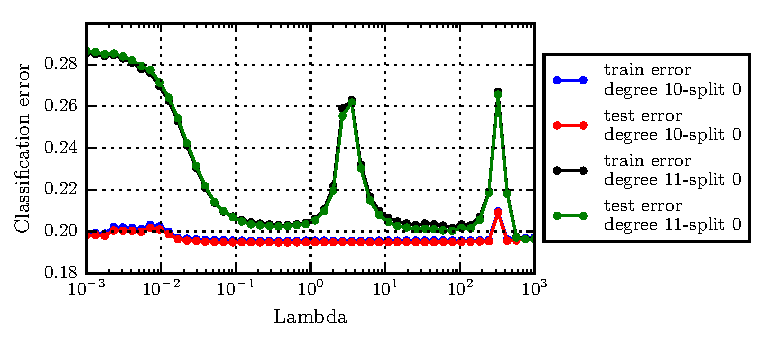
\includegraphics[scale=.7]{Cross_validation_10_11}
	\caption{Cross-Validation for the split $0$ for polynomials of degree $10$,$11$ and $\lambda$ ranging from $10^{-3}$ to $10^3$.}
	\label{fig:cross-validation}
\end{figure}

We have here in our figure a behaviour that could seem strange, because the cross-validation plot has peaks, and is flat otherwise. It is due to the fact we do not use a cost function here, but that we rather compute the classification error (in percentage of error). We know that a small cost function implies a small classification error, but we also know that the converse is not true : a small classification error will not imply a small cost function. Hence, the graph that we have here can seem quite unpredictable. We choose to use the classification error over to usual cost function because it allowed for searching for a wider range of solutions : some that would not minimize the cost function, but would actually classify our data quite well.
\section{Conclusion}
We were able to approach the problem of finding the Higgs Boson from with quite different Machine Learning methods, but were very surprised in the result. While we expected the (Regularized) Logistic Regression to perform well, it presented too many fallbacks for us to use it reliably : the convergence was very slow, the result not extremely accurate. We used then the Ridge regression, which isn't iterative, and obtained our best predictions with it.
\end{document}
